\documentclass[11pt,nswissgerman]{article}
\usepackage{helvet}
\renewcommand{\familydefault}{\sfdefault}
\usepackage[latin2]{inputenc}
\usepackage[a4paper]{geometry}
\geometry{verbose,tmargin=3cm,bmargin=3cm,lmargin=3.5cm,rmargin=3.5cm,headheight=3cm,headsep=1cm,footskip=2cm}
\usepackage{fancyhdr}
\pagestyle{fancy}
\usepackage{wrapfig}
\usepackage[draft]{graphicx}
\usepackage[position=bottom]{subfig}
\usepackage{titletoc}
\usepackage{lipsum}
\makeatletter
\@ifundefined{date}{}{\date{}}
\makeatother
\usepackage{babel}



\setcounter{secnumdepth}{1} % levels under \section are not numbered
\setcounter{tocdepth}{2}    % levels under \subsection are not listed in the TOC



\begin{document}
\begin{titlepage}
\centering

\includegraphics[width=10cm]{../Bilder/Logo/Logo.png} \\
\vspace{2cm}
{\huge\bfseries Gesammelte Werke von jackthebus.com\par}
\vspace{2cm}
{\large Stefan Bopp} \\
{\large Chantal Frunz}
\vfill
{\Large V1.1}
\thispagestyle{empty}

\end{titlepage}
\newpage




\tableofcontents

\newpage

\lhead{Dolomiten 2014}

\rhead{jackthebus.com}

\cfoot{\thepage}
%    JJJ    AA     CCCCCC KKK   K TTTTTT HH  HH EEEEEE BBBBBB UU  UU SSSSSS    CCCCCC OOOOOO MM  MM
%    JJJ   AAAA    CCCCCC KKK  K  TTTTTT HH  HH EEEEEE BB   B UU  UU SSS       CCCCCC OOOOOO MM  MM
%    JJJ  AA  AA   CC     KKK K     TT   HHHHHH EEE    BB   B UU  UU SSS       CC     OO  OO MMMMMM
%    JJJ AA    AA  CC     KKKK      TT   HHHHHH EEEEEE BBBBBB UU  UU  SSSSS    CC     OO  OO M MM M
%    JJJ AAAAAAAA  CC     KKK K     TT   HH  HH EEE    BB   B UU  UU    SSS    CC     OO  OO M MM M
% JJJJJJ AA    AA  CCCCCC KKK  K    TT   HH  HH EEEEEE BB   B UUUUUU    SSS .. CCCCCC OOOOOO M MM M
% JJJJJJ AA    AA  CCCCCC KKK   K   TT   HH  HH EEEEEE BBBBBB UUUUUU SSSSSS .. CCCCCC OOOOOO M MM M
% 
% Texte Geschrieben von Stefan Bopp und Chantal Frunz
% Mehr Informationen sind auf jackthebus.com zu finden
%
\subsection{07.07.2014 Abfahrt und Ankunft}

\begin{wrapfigure}{R}{0.45\textwidth} 
  \begin{center}
    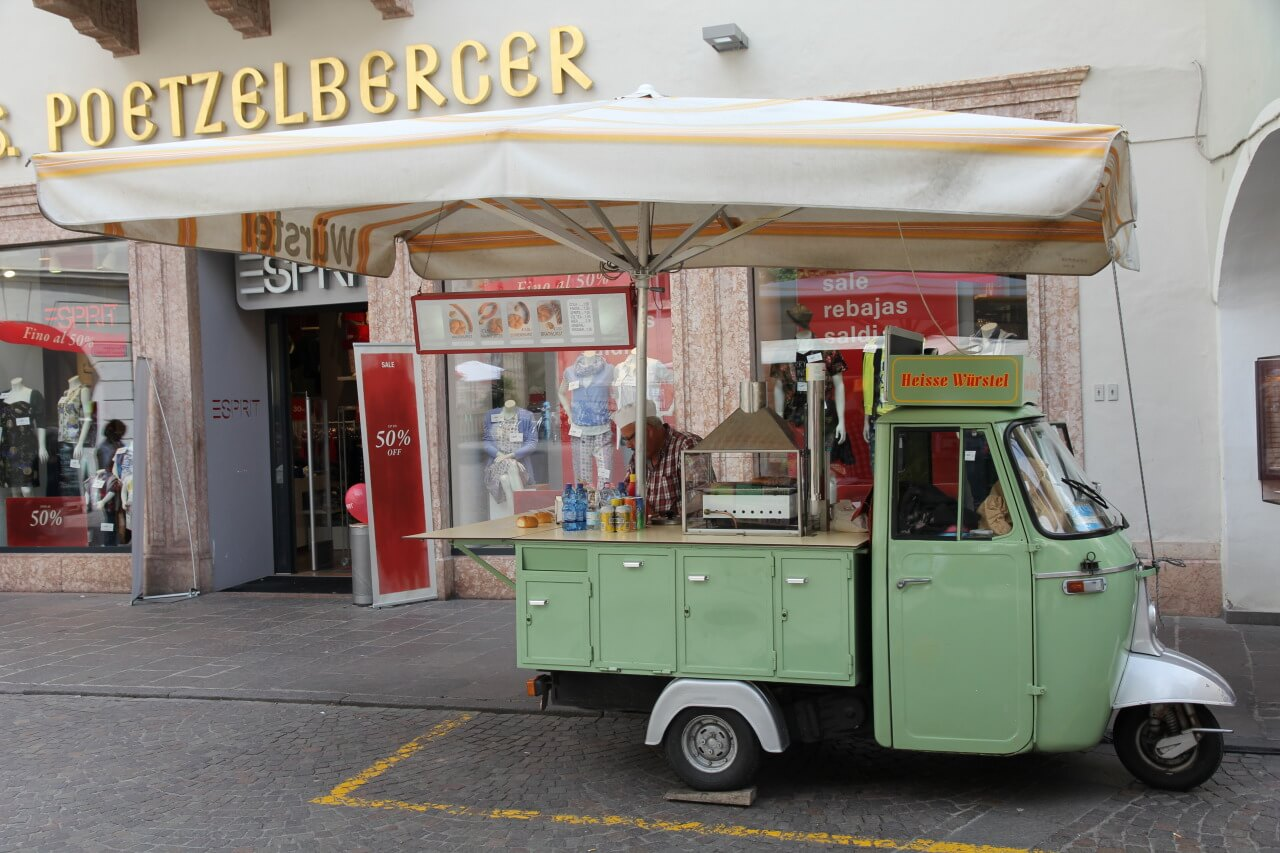
\includegraphics[width=0.4\textwidth]{../Bilder/Dolomiten/2.jpg}
    \caption{GOGOL}
  \end{center}
\end{wrapfigure} 
\lipsum[1-4]

Schon fr�h um 5 Uhr klingelte der Wecker und l�utete gleichzeitig eine neue Episode des Busreisens ein.
Das Ziel ist: Toblach, Dolomiten, Italien.
Der Wetterbericht verhiess nichts gutes und leider folgte das Wetter auch noch dem Bericht.
Die Velos mussten noch auf den modifizierten Paulchen gebunden werden, was auch unter reichlichem Protest von Seiten des Himmels geschah.
Kurz nach 6 Uhr waren wir auf dem Weg Richtung S�dtirol.
Route: Hirzel, Landquart, Davos, Fl�ela, Ofenpass, Meran, Bozen, Toblach.
Schon kurz nach Luzern steigerte sich der Regen und es wurden gewisse Erinnerungen an Korsika wach.
Um 9 Uhr war der erste Halt mit Verpflegung in Davos.
Dieser wurde sogleich auch genutzt um die Vorr�te aufzustocken.
Tapfer ginge es weiter �ber Fl�ela geradewegs in den Schweizer Nationalpark.
Wie bestellt, besserte sich das Wetter und gab den Blick frei auf die wundersch�ne wilde Landschaft.
Nach einigen Fotostopps meisterten wir auch den Ofenpass und bald konnten wir die unz�hligen Schl�sser und Burgen des S�dtirols sehen.
Nach einer langen Fahrt durch Obstbaumplantagen kamen wir in Meran an, wo Chantal sogleich ihrem Hobby nachgehen wollte (Es kann sich jeder selber denken um was es da wohl geht).
Nach dem erfolgreich das Stadtzentrum gefunden wurde, fanden wir auch einen Parkplatz.
Ein Fund, welcher uns sofort verdorben worden ist.
Ein Anwohner steuerte auf uns zu und warnte uns davor, dass an dieser Strasse immer wieder Diebst�hle geschehen.
Vielen Dank f�r den Hinweis, wird aber eiskalt ignoriert!  Parkticket gel�st und schon fast unterwegs als ein Auto neben uns stoppt und die Fahrerin macht uns darauf aufmerksam, dass hier hie und da gerne einmal ein Auto aufgebrochen wird.
Wieder ignorieren oder sich doch langsam Gedanken machen? Wir beschlossen dann einen anderen Parkplatz aufzusuchen.
Nach einem herrlichen Mittagessen (Wolfsbarschfilet mit Hausgemachten Kroketten und Tagliatelle an Zitronensauce mit Crevetten) schlenderten wir durch die Gassen von Meran und der weibliche Teil ging der Jagd nach Lederartigem nach.
Gl�cklicherweise fanden wir dann ein Gesch�ft, welches sogar wirklich sch�ne Taschen verkaufte und ich konnte endlich Ersatz f�r die geklaute, geschenkte (oder umgekehrt) Tasche von unserem Italien Abenteuer beschaffen.
Oha, Warnung vor dem Parkplatz und auch wieder eine Ledertasche! Sehr unsch�ne Erinnerungen.

\begin{figure}[hb]
   \centering
      %\subfloat[CAPTION]{BILDERCODE}\qquad
      \subfloat[GOGOL]{\rule{0.3\textwidth}{2cm}}\quad
      \subfloat[GOGOL]{\rule{0.3\textwidth}{2cm}}\quad
      \subfloat[GOGOL]{\rule{0.3\textwidth}{2cm}}
   \caption[Titel des Bildes]{Titel des Bildes}
\end{figure}

Die weitere Fahrt verlief relativ Ereignislos und auf einmal zeigten sich die ersten charakteristischen Zacken am Horizont.
Diese verschwanden jedoch genauso schnell wieder und irgendwie glich die Landschaft eher Ober-Ehrendingen als den Dolomiten.
Doch kurz vor dem eigentlichen Ziel lugten die majest�tischen Bergspitzen wieder hervor.
Auf dem Campinplatz Olympia schlugen wir unserer Bus auf und kurz nachdem ich die Velos vom Bus entladen hatte, kam auch schon ein �lterer Herr auf mich zu und warnte mich vor Velodieben.
WHAAAT.
Hier schon wieder??  Ignorieren und Velos abschliessen war die Devise.
Nach einem Ap�ro stand der Besuch des Restaurants an.
Beim des Esstempels empfing uns schon der angek�ndigte Regen.
Schnell in den Bus.
Der Niederschlage begleitete uns mit Blitz und Donner in den Schlaf.

Die Sonne gr�sste uns als wir nach einer erholsamen Nacht aus dem Bus krochen.
Schnell denn Camping-Shop besucht und schon waren wir auch mit Gipfeli und Br�tli versorgt.
Der Wetterbericht versprach jedoch vor allem eines: Wasser.
Darum war der Plan nach Bruneck zu gehen und den Tag mit Shoppen zu verbringen.
Schon beim zusammenr�umen der Sachen wurde das Wetter noch tr�ber.
Auch die Spitzen der Berge haben sich hinter den Nebel zur�ckgezogen.
Nach einer halben Stunde Fahrt durch heftigen Regen kamen wir in Bruneck an und fanden sogleich ein Parkplatz (Diese Mal ohne Warnung vor Dieben).
Das erste Lokal war sogleich das Speckmuseum.
Bl�d aber auch.
Die Zeit verging wie im Fluge und manche Gesch�fte wurden besucht und dies und das eingekauft.
Auch ein Ap�ro durfte nat�rlich nicht fehlen und schon bald verschlechterte sich das Wetter wieder, nachdem es denn ganzen Nachmittag eigentlich nie richtig schlecht war.
Im str�menden Regen ging es zur�ck zu Jack.
Auf der Fahrt zur�ck verbesserte sich das Wetter noch einmal, jedoch wurde es empfindlich kalt.
Als Abendessen diente die Beute aus Bruneck und grosse Pl�ne f�r den n�chsten Tag wurden geschmiedet.
Trotz eher m�ssigen Wetters sollten die drei Zinnen umrundet werden.
Traditionsgem�ss liessen wir denn Tag mit der 3. Staffel Homeland ausklingen.
Brasilien wurde am selben Abend mit 7:1 ausgeklungen, heftig!

\subsection{09.07.2014 Im Fr�htau zu Berge...}

\begin{wrapfigure}{R}{0.30\textwidth} 
  \begin{center}
      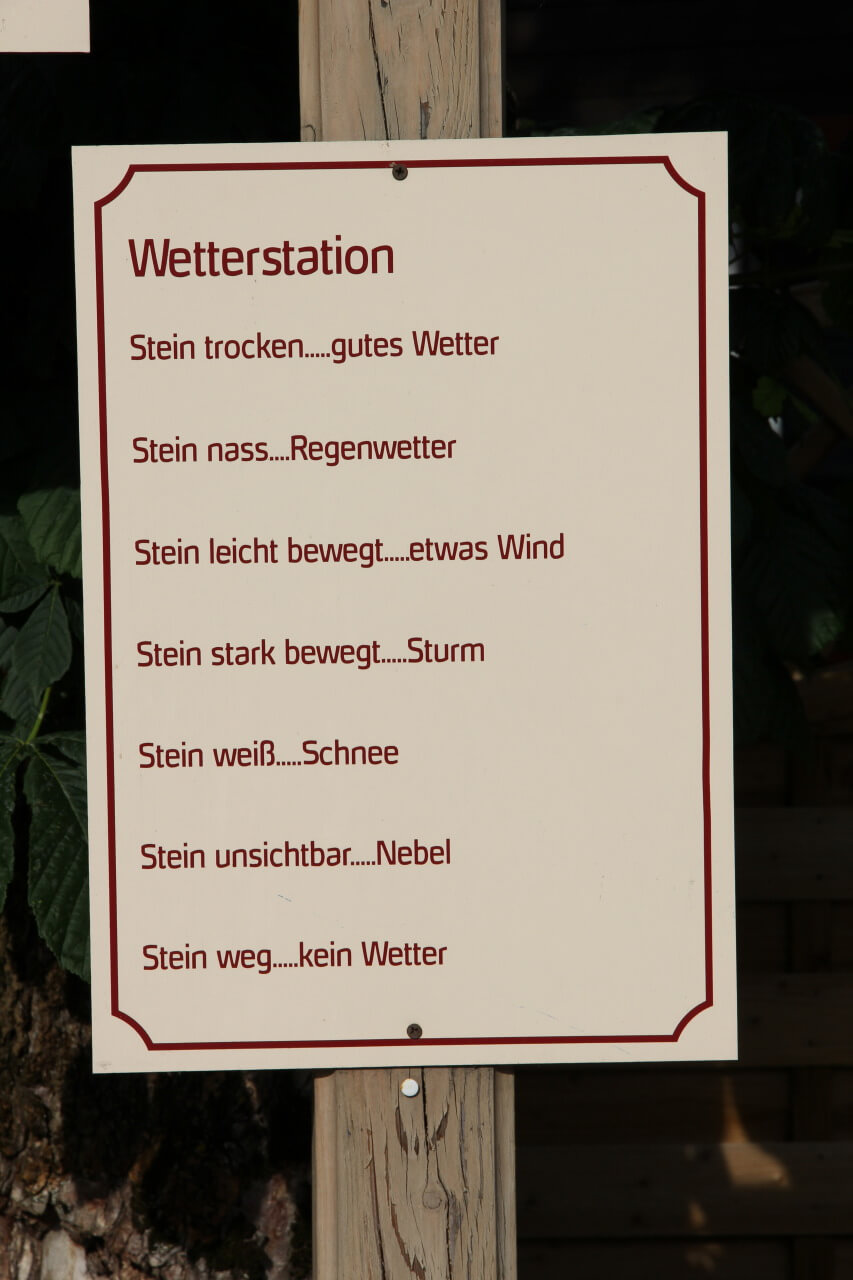
\includegraphics[width=0.4\textwidth, height=5cm,keepaspectratio]{../Bilder/Dolomiten/6.jpg}
    \caption{GOGOL}
  \end{center}
\end{wrapfigure} 

Nach einer k�hlen Nacht, 9\textdegree C im Juli, wurden wir von einer kurzen Regenpause aus dem Bus gelockt. Nach einem k�hlen Fr�hst�ck konsultierten wir nochmals den Wetterbericht, welcher auch nicht gerade mit guten News um sich warf. Schneefallgrenze sank gegen 2000m. Trotz allen Widrigkeiten stiegen wir in die Wandersachen und wollten nun endlich die ber�hmten drei Zinnen aus der N�he betrachten. Nach einer halbst�ndigen Fahrt, stets bergauf, stoppte uns eine Barriere. Das ganze sah irgendwie wie ein verirrtes Zollhaus aus. Bei der Barriere angehalten meinte der Typ irgendetwas mit Zwanzig und Vier. Aha, der wollte Kohle. Vermutlich um sein H�uschen mitten auf der Strasse zu finanzieren. Na gut, geben wir dem halt 4 Euro 20. Doch halt, er machte noch einmal auf sich aufmerksam und sagte jetzt deutlicher: �24 Euro bitte.� Gopferdeckel, Na gut jetzt sind wir schon mal hier. Weiter ging die Fahrt sehr steil bergauf. Der Zeiger der Wassertemperatur lehnte sich schon verd�chtig weit nach rechts als endlich der ersehnte Parkplatz in Sichtweite kam. Wir befanden uns jetzt auf 2300 Meter �ber Meer. �berall um uns herum befanden sich nun die spitzigen T�rme der Dolomiten und auch das Wetter hatte kurz Erbarmen und die Wolkendecke �ffnete sich ein St�ck. Es war jedoch A...kalt. Wir packten uns mit allem ein was wir dabei hatten und machten uns auf den Weg rund um die drei Zinken. Zuerst noch bei halbwegs gem�tlichem Wetter, der letzte Drittel dann bei Graupel. Eine kurze Rast in einer Bergh�tte brachte leider keine Besserung, daf�r ein Bier und so waren wir froh als wir wieder den Parkplatz erreichten, wo Jack mit einer Heizung und trockene Kleidung wartete. Die Fahrt zur�ck verlief problemlos und auf dem fast schon heimischen Campingplatz angekommen, war es Zeit f�r eine Pause. Kurz darauf zeigte sich jedoch die Sonne und so sattelten wir die Velos, welche bis jetzt eher Schmuck als Fahrzeug waren, und radelten Richtung Toblach. Das kleine D�rfchen war schneller erkundet als den Ortsnamen ausgesprochen. Nach einem Campari fanden noch ein Rindsfillet sowie ein Wienerschnitzel r�bis und st�bis den Weg in die M�gen. 

\subsection{10.07.2014 Nudelfertig}
Unser Hauptthema, das Wetter spielte ein weiteres Mal nicht so mit, wie wir uns das so vorstellten.
Nieselregen und Temperaturen im einstelligen Bereich luden nicht gerade zu einer Velotour ein.
Trotzdem kleideten wir uns dem Wetter entsprechend und machten uns Testweise Richtung Toblachersee auf den Weg.
Trotz ausbleibender Wetterverbesserung beschlossen wir weiter zu fahren.
Im dem Wasser entlang ging es nach Cortina d'Ampezzo.
Eine wundersch�ne Route, welche jedoch durch das Wetter ein wenig getr�bt worden ist.
Viele Velofahrer und E-Biker waren unterwegs, da am Wochenende ein Bikerennen stattfinden sollte.
Die aus gesteckte Wasserdurchfahrt wurde mehrfach getestet, was mit ein wenig Stolz und umso feuchtere Schuhe endete.
Der Aufstieg zog sich in die L�nge und Chantal musste auf einmal einen ungeplanten Stopp einlegen (\dots ).
Solange der Weg leicht anstieg war die K�lte noch relativ gut ertr�glich, dies �nderte sich jedoch mit der Abfahrt z�gig.
Bis nach Cortina froren mir fast die nassen Flossen ab, das fehlende Mittagessen half in diesem Moment auch nicht gerade.
Viel Spass beim Mittagessen suchen um 15:00 Uhr.
Der Bus, welcher uns zur�ck nach Toblach bringen sollte fuhr um 16:00 und so waren wir kurz nach 17:00 schon wieder zur�ck.
Nudelfertig und hungrig machten wir uns nach 2 Stunden Pause besuchten wir das Nachbardorf Niederdorf und fanden schon nach kurzer Zeit ein passendes Restaurant f�r den letzten Abend.
Ochsenfillet stand auf der Karte, welches auch hervorragend schmeckte.

\begin{figure}
    \centering
    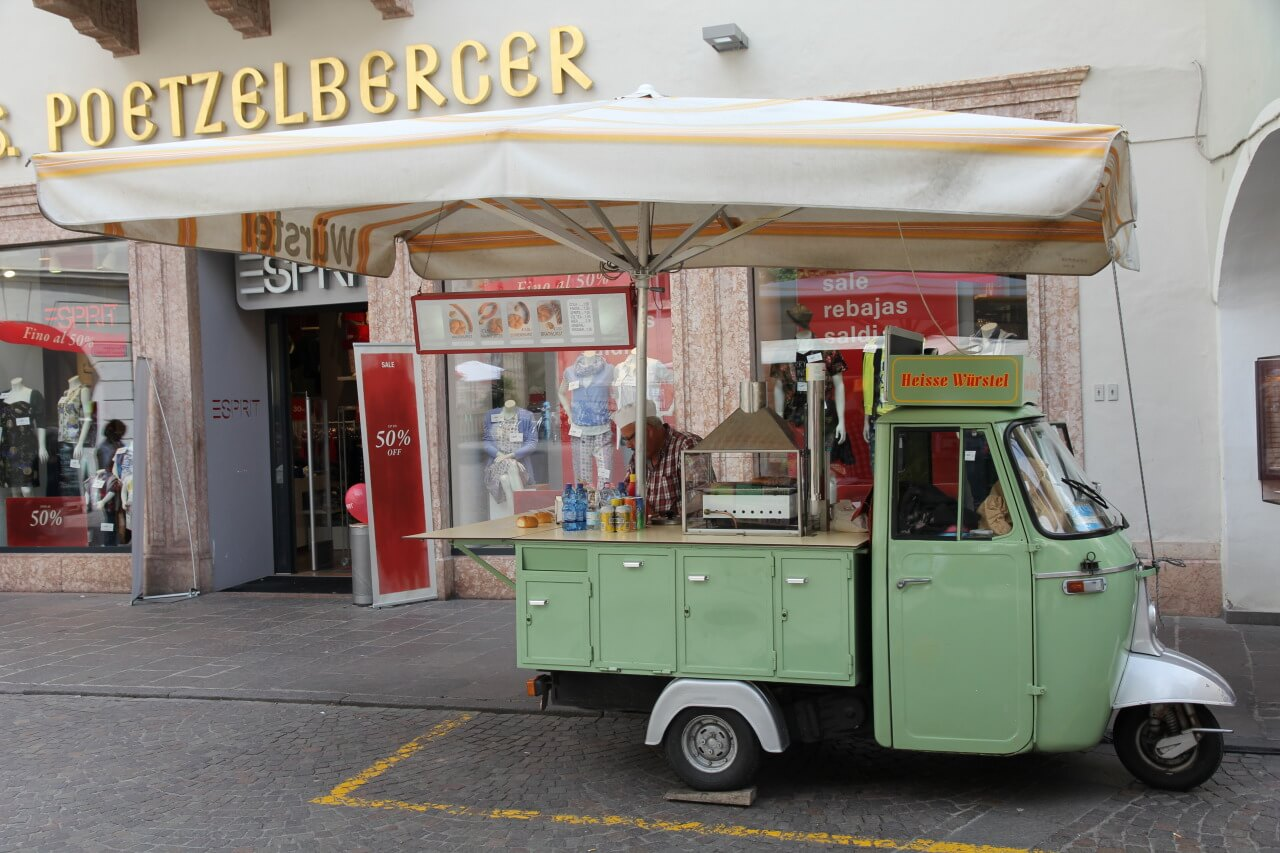
\includegraphics[width=\textwidth]{../Bilder/Dolomiten/2.jpg}
    \caption{eine Grafik ohne Sinn}
    \label{img:grafik-test}
\end{figure}

\subsection{11.07.2014 Wo ist er denn?}
Schon vor 9 Uhr waren wir auf den Beinen um die Abreise vorzubereiten und routiniert ging alles von statten bis ich die Velos aufladen wollte.
Wo ist der bl�de Schl�ssel hingekommen.
Fluchen, Rekonstruieren und Suchen brachten nichts.
Also mit wenig Hoffnung machte ich mich daran mit dem Seitenschneider das Schloss zu bearbeiten.
Chantal fragte an der Rezeption derweilen nach etwas h�rterem Gesch�tz.
Zu unser aller �berraschung liess sich das Schloss jedoch innerhalb von 1.
5 Minuten mit einem einfachen Seitenschneider �ffnen.
Ein Gl�ck das niemand anderes das Gleiche vor uns versucht hat.
Endlich auf dem Weg ging es zum Fr�hst�ck ein weiteres Mal nach Bruneck.
Noch einmal ein Besuch im Speckmuseum ein kurzes Fr�hst�ck und nichts mehr stand zwischen uns und Innsbruck.
Naja, der Brenner musste noch bezwungen werden.
Aber auch dieser stellte kein richtiges Hindernis dar und so waren wir schon bald angekommen.
Mittel Park und Ride gelangen wir ins Stadtzentrum.
Schnell wurden die �blichen verd�chtigen Shops besucht und gegen 16:00 machten wir uns auf den Weg den Rest der Strecke nach Luzern unter die R�der zu nehmen.
Das Wetter war im S�dtirol noch wundersch�n, in der Schweiz empfing uns dann wieder das gleiche Wetter wie bei er Abfahrt.
Heftiger Regen.
Kurz nach 20:00 waren wir mit zwei Take-Away Pizzas zur�ck in der Wohnung. 


\end{document}
